
%\title{User guide to the alchemical free energy perturbation 
%       calculations in NAMD}

This feature has been contributed to \NAMD\ by the following authors:

\begin{quote}
   Surjit B. Dixit and Christophe Chipot          \\[0.4cm]
   {\it Equipe de chimie th\'eorique,                 }\\
   {\it Institut nanc\'eien de chimie mol\'eculaire,  }\\
   {\it UMR {\sc Cnrs/Uhp} 7565,                      }\\
   {\it Universit\'e Henri Poincar\'e,                }\\
   {\it BP 239,                                       }\\
   {\it 54506 Vand\oe uvre--l\`es--Nancy cedex, France}
\end{quote}

%\date{\small Version: \today 
%\\[10.2cm]
%\copyright~2001, {\sc Centre National de la Recherche Scientifique}}


\subsubsection{Introduction and theoretical background}


A method to perform alchemical free energy perturbation (\FEP)
~\cite{zwan_54_1,Beveridge.89,Gunsteren.89,Straatsma.92,Kollman.93,Gilson.97,
Mark.98,chip_01_1} within \NAMD\ has now been implemented. 
Within \FEP, the difference in free energy between two states,
$a$ and $b$, is expressed by:

\begin{equation}
\Delta A_{a \rightarrow b} = -k_B T \ \ln
\left< \exp\left[-\frac{{\cal H}_b({\bf r}, {\bf p}) - 
                         {\cal H}_a({\bf r}, {\bf p})}
                        {k_B T}\right]
\right>_a
\end{equation}

wherein $k_B$ is the Boltzmann constant, $T$ is the kinetic temperature,
and ${\cal H}_a({\bf r}, {\bf p})$ and ${\cal H}_b({\bf r}, {\bf p})$
are the Hamiltonians characteristic of states $a$ and $b$, respectively.
$\left< \cdots \right>_a$ denotes an ensemble average over configurations
representative of the initial state, $a$.
In practice, the transformation between the two thermodynamic states
is replaced by a series of transformations between non--physical,
intermediate states along a pathway that connects $a$ to $b$.
This pathway is characterized by a variable, referred to as
``coupling parameter'',~\cite{Beveridge.89,Mark.98,king_93_1} 
$\lambda$, that makes the free energy
a continuous function of this parameter between $a$ and $b$:

\begin{equation}
\Delta A_{a \rightarrow b} = -k_B T \ \sum_{k = 1}^N \ln
\left< \exp\left[-\frac{{\cal H}({\bf r}, {\bf p}; \lambda_{k+1}) - 
                         {\cal H}({\bf r}, {\bf p}; \lambda_k)}
                        {k_B T}\right]
\right>_k
\end{equation}

Here, $N$ stands for the number of intermediate states, or ``windows''
between the initial and the final states.


In a typical \FEP\ setup involving the transformation
of one chemical species into another one in the course 
of the simulation, the atoms in the molecular topology can be 
classified into three groups. A group of atoms that do not change 
during the simulation --- \eg the environment,  
the atoms describing the initial state, $a$, of the system, and, last, the 
atoms that correspond to the final state, $b$, at the end of the 
alchemical transformation. 
The excluded pairs are defined in the {\tt psf} file, so that 
the atoms representative of state $a$
do not interact with those of state $b$ throughout the 
entire molecular dynamics ({\sc md}) simulation. 
Such a setup, in which atoms of both the initial and the
final states of the system are present in the molecular topology file --- \ie 
the {\tt psf} file --- is characterisitic of the so--called ``dual topology'' 
protocol.~\cite{Axelsen.98}
The hybrid Hamiltonian of the system, which is a function of the
coupling parameter $\lambda$, that smoothly connects state $a$
to state $b$, is calculated as:

\begin{equation}
{\cal H}(\lambda) = {\cal H}_0 + \lambda {\cal H}_a + (1-\lambda) {\cal H}_b
\end{equation}

where ${\cal H}_a$ is the Hamiltonian of the group of atoms representative
of the initial state, $a$, and ${\cal H}_b$ characterizes the final state,
$b$. 
${\cal H}_0$ is the Hamiltonian for those atoms that do not undergo any 
transformation during the {\sc md} simulation.


In the present implementation of \FEP\ in \NAMD, we employ a hamiltonian
scaling procedure as is done in the ``dual topology''
approach,~\cite{Pearlman.93} \ie instead 
of scaling the non--bonded parameters of states $a$ and $b$, 
namely the net atomic charges, together with the Lennard--Jones parameters, 
as a function of the coupling parameter, $\lambda$:

\begin{eqnarray}
\nonumber
q_i &=& \lambda_i \ q_i \\[0.4cm]
\epsilon_{ij} &=& \sqrt{\lambda_i \ \epsilon_{ii} \ \lambda_j \ \epsilon_{jj}} \\[0.4cm]
\nonumber
\sigma_{ij} &=& \frac{\lambda_i \ \sigma_{ii} + \lambda_j \ \sigma_{jj}}{2} 
\end{eqnarray}

where $\lambda_i$ and $\lambda_j$ take the value of $\lambda$ or $(1-\lambda)$,
depending upon state $a$ or $b$, to which $i$ or $j$ belong.


For instance, in a transformation involving the mutation of an
alanine side chain into that of glycine, using the \FEP, the topology
of both the methyl group borne by the C$_\alpha$ in alanine,
and the hydrogen of glycine co--exist throughout the simulation
(see Figure~\ref{fig:dual_top}).


\begin{figure}[ht]
  \center{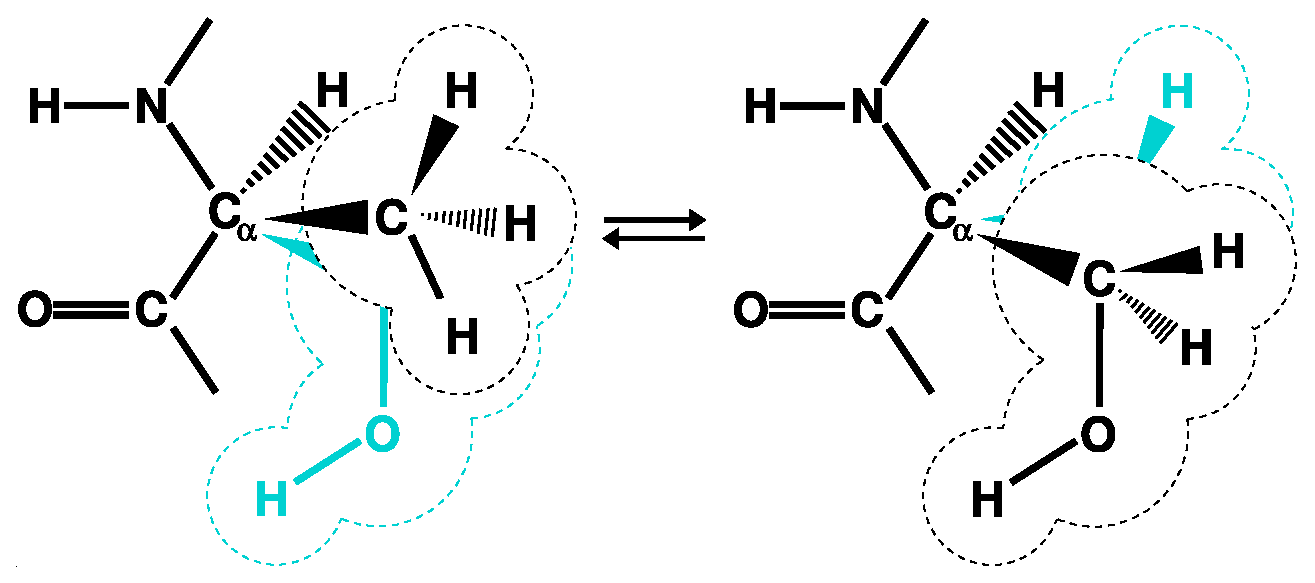
\includegraphics[width=14.5cm]{figures/dual_top}}
  \caption{Dual topology description for an alchemical simulation.
         Case example of the mutation of alanine into glycine.
         The lighter color denotes the non--interacting, alternate
         state.}
  \label{fig:dual_top}
\end{figure}


The charge and Lennard--Jones parameters of the alanine and
the glycine side chains
are defined as a function of $\lambda$, in such a fashion that 
the interaction of the methyl group of alanine with the rest of 
the protein is effective at the beginning of the simulation,
\ie $\lambda$ = 0, while
the glycine C$_\alpha$ hydrogen does not interact with the rest
of the protein, and {\it vice versa} at the end of the
simulation, \ie $\lambda$ = 1.
For intermediate values of $\lambda$, both the alanine and the glycine
side chains participate in non--bonded interactions with the rest 
of the protein, scaled on the basis of the current value of $\lambda$.
It should be emphasized that these side chains, however,
do not interact with themselves. Explicit care should be taken while
preparing the {\tt psf} file to exclude those atoms that are created
from those that will be annihilated in the course of the
\FEP\ calculation.


It is also worth noting that
the free energy calculation does not alter intramolecular
potentials, \ie bond stretch, valence angle deformation, torsions,
{\it etc}\dots, during
the simulation. In calculations targetted at the estimation
of free energy differences between two states characterized by
distinct environments --- \eg a ligand, bound to a protein in
the first simulation,
and solvated in water, in the second --- as is the 
case for most free energy calculations that make use of a thermodynamic 
cycle, perturbation of intramolecular terms can be safely
avoided.~\cite{Boresch.99a}


\subsubsection{Implementation of free energy perturbation in NAMD}


The procedure implemented in \NAMD\ is particularly
adapted for performing free 
energy calculations that split the $\lambda$
reaction path into a number of non--physical,
intermediate states, or ``windows''. Seperate simulations 
can be started for each window.
Alternatively, the {\sc Tcl} scripting ability of 
\NAMD\ can be employed advantageously
to perform the complete simulation in a single run.
An example making use of such script is supplied at the end 
of this user guide.


The following keywords can be used to control the alchemical free 
energy calculations. 

\begin{itemize}

\item
\NAMDCONFWDEF{fepOn}{ Is alchemical \FEP\ to be performed? }
{{\tt on} or {\tt off}}
{{\tt off}}
{Turns on parameter scaling and ensemble averaging for alchemical \FEP.}

\item
\NAMDCONF{lambda}{ Coupling parameter value }
{positive decimal between 0.0 and 1.0}
{The coupling parameter value determining the progress of the
perturbation. The non--bonded parameters of the atoms vanishing
in the course of the {\sc md} simulation are scaled by {\tt lambda}, whilst
the parameters of those atoms grown are scaled by (1-{\tt lambda}).}

\item
\NAMDCONF{dLambda}{Coupling parameter step}
{positive decimal between 0.0 and 1.0}
{The {\tt dLambda} value corresponds to the magnitude of the change in
the coupling parameter, $\lambda$, that defines the spacing between
adjacent windows.}

\item
\NAMDCONFWDEF{numFepEqlb}{Number of equilibration steps in the window, 
before data collection}
{positive integer less than {\tt numSteps} or {\tt run}}
{0}
{In each window {\tt numFepEqlb} steps of equilibration can be
performed before ensemble averaging is initiated. The output also contains
the data gathered during equilibration and is meant for analysis of
convergence properties of the \FEP\ calculation.}

\item
\NAMDCONFWDEF{fepFile}{{\sc pdb} file with perturbation flags}
{{\sc Unix} filename}
{coordinates}
{{\sc pdb} file to be used for indicating the \FEP\ status for each of
the atoms pertaining to the system. 
If this parameter is not declared specifically, then the
{\sc pdb} file containing the initial coordinates specified by
{\tt coordinates} is utilized for this information.}

\item
\NAMDCONFWDEF{fepCol}{Column in the {\tt fepFile} that carries 
                      the perturbation flag}
{X, Y, Z, O or B}
{O}
{Column of the {\sc pdb} file to use for retrieving the \FEP\ status 
of each atom, \ie a flag that indicates which atom will be perturbed
in the course of the simulation.
A value of {\tt -1} in the specified column indicates the atom will
vanish during the \FEP\ calculation, whereas a value of {\tt 1} 
indicates that the atom would grow.}

\item
\NAMDCONFWDEF{fepOutFreq}{Frequency of \FEP\ energy output in time--steps}
{positive integer}
{5}
{Every {\tt fepOutFreq} number of {\sc md} steps, the output file
{\tt fepOutFile} is updated by dumping energies that are
used for ensemble averaging.
This variable could be set to {\tt 1} to include all the 
configurations for ensemble averaging. Yet, it is recommended
to update {\tt fepOutFile}  energies with a
higher frequency 
to avoid large correlation between consecutive configurations.}

\item
\NAMDCONFWDEF{fepOutFile}{\FEP\ energy output filename}
{filename}
{outfilename}
{An output file named {\tt fepOutFile}.fep, generated by \NAMD,
contains the \FEP\ energies, dumped every {\tt fepOutFreq} steps.}

\item
\NAMDCONFWDEF{scaleH}{Perform Hamiltonian scaling }
{{\tt on} or {\tt off}}
{{\tt on}}
{Presently NAMD can perform Hamiltonian scaling based FEP simulation.
Amber (xleap) generated perturbation prmtop file is not supported
and parameter scaling based calculation cannot be performed with this
version.}

\end{itemize}


\subsubsection{Examples of input files for running FEP alchemical calculations}


The first example illustrates the use of {\sc Tcl} scripting for running
the alchemical \FEP\ feature of \NAMD: 

\begin{verbatim}
fepOn		on  
fepfile		ion.fep
fepCol		X
fepoutfile	ion.fepout
fepOutFreq	5
numFepEqlb	5000

set step 0.0
set dstep 0.1

while {$step <= 0.9} {
 firsttimestep	0
 lambda $step
 dlambda $dstep
 run  10000
 set step [expr $step+$dstep]
}
\end{verbatim}

Here, the {\sc pdb} file read by \NAMD\ to retrieve the information
about perturbed atoms is {\tt biotin.fep}. The pertinent information 
is present in the {\tt X} column. The output file of the free energy
calculation is {\tt biotinr.fepout}, in which energies are written
every {\tt 5} steps. No electrostatic decoupling is employed. 
$\delta \lambda$, the width of the windows, is set to {\tt 0.1}.
{\tt 5000} {\sc md} steps are performed in each window to
equilibrate the system. In this particular instance, 
the current value of $\lambda$
is controlled by the syntax {\tt set step}. 
The \FEP\ calculation is run until $\lambda$ reaches the
value {\tt 0.9}. In every window, {\tt 10000} {\sc md} steps
are being performed. At each value of $\lambda$, the first 
{\sc md} step is reset to {\tt 0} by means of the command
 {\tt firsttimestep}.


In the second example, each $\lambda$--state is declared
explicitly, avoiding the use of {\sc Tcl} scripting:

\begin{verbatim}
fepOn		on  
fepfile		ion.fep
fepCol		X
fepoutfile	ion.fepout
fepOutFreq	5
dLambda		0.1
numFepEqlb	5000

Lambda		0.0
run		10000

lambda		0.1
firsttimestep	0
run		10000
\end{verbatim}
$\vdots$
\begin{verbatim}
lambda		0.8
firsttimestep	0
run		10000

lambda		0.9
firsttimestep	0
run		10000
\end{verbatim}

The \FEP\ calculation is carried out from $\lambda$ = {\tt 0.0} to
{\tt 0.9}. In each new window, {\tt 10000} {\sc md} steps are
performed, and the number of steps is being reinitialized using
the {\tt firsttimestep} keyword.



\subsubsection{Description of \FEP\ simulation output }

The {\tt fepOutFile} contains electrostatic and van der Waals energy
data calculated for $\lambda$ and $\delta\lambda$, written every
{\tt fepOutFreq} steps. The column {\tt dE} is the energy
difference of the single configuration, {\tt dE\_avg} and {\tt dG}
are the instantaneous ensemble average of the energy and the calculated
free energy at the time step specified in column 2, respectively.
The temperature is specified in the penultimate column. On completion
of {\tt numFepEqlb} steps, the calculation of {\tt dE\_avg} and 
{\tt dG} is restarted. The accumulated net free energy change is output
and the end of the simulation at each lambda value. The cummulative
average energy {\tt dE\_avg} value may be summed using the 
trapezoidal rule to obtain an approximate TI estimate for the free 
energy change during the run.


